% Options for packages loaded elsewhere
\PassOptionsToPackage{unicode}{hyperref}
\PassOptionsToPackage{hyphens}{url}
%
\documentclass[
]{article}
\usepackage{amsmath,amssymb}
\usepackage{iftex}
\ifPDFTeX
  \usepackage[T1]{fontenc}
  \usepackage[utf8]{inputenc}
  \usepackage{textcomp} % provide euro and other symbols
\else % if luatex or xetex
  \usepackage{unicode-math} % this also loads fontspec
  \defaultfontfeatures{Scale=MatchLowercase}
  \defaultfontfeatures[\rmfamily]{Ligatures=TeX,Scale=1}
\fi
\usepackage{lmodern}
\ifPDFTeX\else
  % xetex/luatex font selection
\fi
% Use upquote if available, for straight quotes in verbatim environments
\IfFileExists{upquote.sty}{\usepackage{upquote}}{}
\IfFileExists{microtype.sty}{% use microtype if available
  \usepackage[]{microtype}
  \UseMicrotypeSet[protrusion]{basicmath} % disable protrusion for tt fonts
}{}
\makeatletter
\@ifundefined{KOMAClassName}{% if non-KOMA class
  \IfFileExists{parskip.sty}{%
    \usepackage{parskip}
  }{% else
    \setlength{\parindent}{0pt}
    \setlength{\parskip}{6pt plus 2pt minus 1pt}}
}{% if KOMA class
  \KOMAoptions{parskip=half}}
\makeatother
\usepackage{xcolor}
\usepackage[margin=1in]{geometry}
\usepackage{longtable,booktabs,array}
\usepackage{calc} % for calculating minipage widths
% Correct order of tables after \paragraph or \subparagraph
\usepackage{etoolbox}
\makeatletter
\patchcmd\longtable{\par}{\if@noskipsec\mbox{}\fi\par}{}{}
\makeatother
% Allow footnotes in longtable head/foot
\IfFileExists{footnotehyper.sty}{\usepackage{footnotehyper}}{\usepackage{footnote}}
\makesavenoteenv{longtable}
\usepackage{graphicx}
\makeatletter
\def\maxwidth{\ifdim\Gin@nat@width>\linewidth\linewidth\else\Gin@nat@width\fi}
\def\maxheight{\ifdim\Gin@nat@height>\textheight\textheight\else\Gin@nat@height\fi}
\makeatother
% Scale images if necessary, so that they will not overflow the page
% margins by default, and it is still possible to overwrite the defaults
% using explicit options in \includegraphics[width, height, ...]{}
\setkeys{Gin}{width=\maxwidth,height=\maxheight,keepaspectratio}
% Set default figure placement to htbp
\makeatletter
\def\fps@figure{htbp}
\makeatother
\setlength{\emergencystretch}{3em} % prevent overfull lines
\providecommand{\tightlist}{%
  \setlength{\itemsep}{0pt}\setlength{\parskip}{0pt}}
\setcounter{secnumdepth}{-\maxdimen} % remove section numbering
\ifLuaTeX
\usepackage[bidi=basic]{babel}
\else
\usepackage[bidi=default]{babel}
\fi
\babelprovide[main,import]{spanish}
% get rid of language-specific shorthands (see #6817):
\let\LanguageShortHands\languageshorthands
\def\languageshorthands#1{}
\ifLuaTeX
  \usepackage{selnolig}  % disable illegal ligatures
\fi
\usepackage{bookmark}
\IfFileExists{xurl.sty}{\usepackage{xurl}}{} % add URL line breaks if available
\urlstyle{same}
\hypersetup{
  pdftitle={Plan de Negocio},
  pdfauthor={Azul Noguera; Patricio Guledjian; Rocio Gonzalez Cingolani; Rafael Cabre},
  pdflang={es-ES},
  hidelinks,
  pdfcreator={LaTeX via pandoc}}

\title{Plan de Negocio}
\usepackage{etoolbox}
\makeatletter
\providecommand{\subtitle}[1]{% add subtitle to \maketitle
  \apptocmd{\@title}{\par {\large #1 \par}}{}{}
}
\makeatother
\subtitle{Link al repositorio:
\url{https://github.com/azulnogueraa/Creacion-de-Empresas}}
\author{Azul Noguera \and Patricio Guledjian \and Rocio Gonzalez
Cingolani \and Rafael Cabre}
\date{2024-04-24}

\begin{document}
\maketitle

{
\setcounter{tocdepth}{3}
\tableofcontents
}
\newpage

\section*{Plan de Negocio}

\subsection{1. Introducción}\label{introducciuxf3n}

\subsubsection{1.1. CNAE (Clasificación Nacional de Entidades
Económicas)}\label{cnae-clasificaciuxf3n-nacional-de-entidades-econuxf3micas}

Educación.

\subsubsection{1.2. Misión}\label{misiuxf3n}

Ofrecer una educación personalizada y de alta calidad a través de la
tecnología, para que las personas puedan aprender de manera eficiente y
efectiva, mejorando la satisfacción de los estudiantes y las tasas de
finalización de los cursos.

\subsubsection{1.3. Visión}\label{visiuxf3n}

Ser la plataforma de educación en línea más grande y reconocida en el
mundo, ofreciendo una amplia variedad de cursos y programas adaptados a
las necesidades de cada estudiante.

\subsubsection{1.4. Valores}\label{valores}

\begin{itemize}
\tightlist
\item
  Calidad
\item
  Innovación
\item
  Personalización
\item
  Eficiencia
\item
  Ética
\end{itemize}

\newpage

\subsection{2. Descripción de la Oportunidad de
Negocio}\label{descripciuxf3n-de-la-oportunidad-de-negocio}

El avance tecnológico ha registrado una trayectoria ascendente sin
precedentes en las últimas décadas. Este progreso ha catalizado una
transformación paralela en el dominio educativo, propulsando el
e-learning a un primer plano en la entrega de conocimiento y
habilidades. La digitalización de la educación no solo ha democratizado
el acceso a la información, sino que también ha ampliado las fronteras
del aula tradicional, permitiendo un aprendizaje más flexible y
autodirigido.

En el vértice de la crisis sanitaria global, la pandemia de COVID-19 se
desempeño como catalizador para una adopción masiva de la educación en
línea. El confinamiento y la interrupción de la enseñanza presencial
urgieron a una migración acelerada hacia plataformas digitales. Según
una encuesta realizada en julio del año 2020 por la escuela de negocios
Online Business School (OBS)\footnote{FUENTE:
  \href{https://marketing.onlinebschool.es/Prensa/Informes/Informe\%20OBS\%20E-learning\%202022.pdf}{OBS
  Business School -El Estudiante Universitario en Línea. Tendencias y
  Perspectivas.}} de España, el 84\% de los 30 países analizados en la
región había elegido internet como uno de sus sistemas de educación a
distancia.

\begin{figure}
\centering
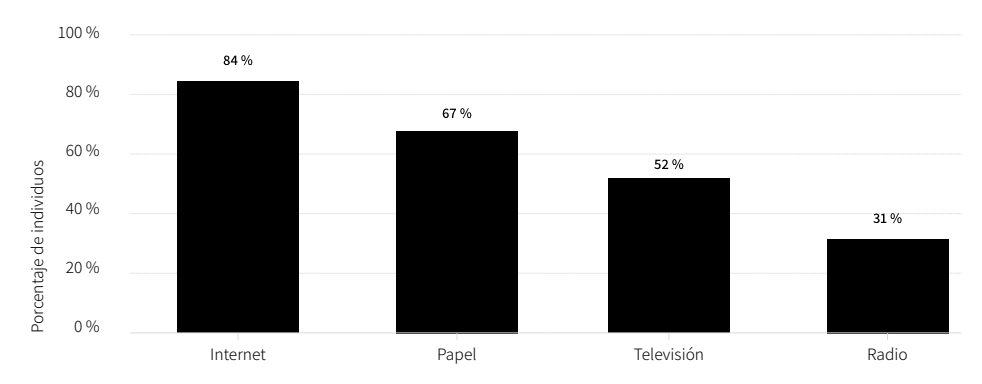
\includegraphics[width=0.7\textwidth,height=\textheight]{img/internet_ante_papel.png}
\caption{Sistemas de entrega de educación a distancia utilizados en
medio de la pandemia de COVID-19}
\end{figure}

Posteriormente, una vez atenuado el impacto directo de la pandemia, la
inercia del aprendizaje en línea perduró. Muchos estudiantes, ahora
acostumbrados al entorno digital, continuaron favoreciendo esta
modalidad, apoyados por la escalada tecnológica que seguía enriqueciendo
esta experiencia. El impulso continuo del e-learning responde también a
una demanda creciente de capacitación constante, vital en un mercado
laboral que se reinventa continuamente. Según estimaciones de Global
Market Insights, la valuación del mercado de e-learning en \$399.3 mil
millones de dolares en 2022 y su proyectado crecimiento a una tasa
compuesta anual del 14\% hasta 2032, subraya esta tendencia.

Sin embargo, el escenario actual de la educación en línea destaca un
marcado contraste entre la disponibilidad de recursos educativos y la
efectividad de su implementación. La mayoría de las plataformas
digitales persisten en ofrecer programas estandarizados, con falta de la
flexibilidad necesaria para atender las demandas personalizadas de
aprendizaje. Esta homogeneización del contenido pedagógico conlleva a
deficiencias en la retención de conocimientos por parte de los
estudiantes, evidenciado por las tasas de finalización de cursos que, de
manera preocupante, suelen rondar el 10\%\footnote{FUENTE:
  \href{https://fastercapital.com/es/contenido/Tasas-de-retencion-de-cursos--Tasas-de-retencion-de-cursos--una-metrica-clave-para-el-exito-del-marketing.html}{fastercapital.com}}.
Tal fenómeno no solo sugiere una desconexión entre la instrucción y la
diversidad de estilos de aprendizaje, sino que también plantea el riesgo
de desaprovechar el potencial académico de estudiantes que requerirían
una metodología más ajustada a sus particularidades. Este desafío en el
panorama educativo actual subraya la necesidad de una plataforma de
aprendizaje electrónico que privilegie la adaptabilidad y
personalización en su oferta curricular, alineándose estrechamente con
las aptitudes y aspiraciones individuales de cada estudiante.

No obstante, investigaciones recientes del año 2023 realizadas por la
Online Business School (OBS)\footnote{FUENTE:\href{https://www.obsbusiness.school/sites/obsbusiness.school/files/media_files/Informe\%20OBS\%20E-Learning\%202023.pdf}{OBS
  Business School - Tendencias y Percepciones sobre la Educación en
  Línea y la Adopción de Tecnologías Educativas}} de España anticipan un
aumento significativo en las inscripciones a programas en línea,
destacando el ámbito de la tecnología con un crecimiento proyectado del
33\% en los próximos cinco años. Esta tendencia subraya una oportunidad
primordial para desarrollar cursos en línea especializados en
tecnología. A continuación, se incluye una figura que ilustra
detalladamente estos hallazgos, fundamentando la viabilidad y el
potencial de esta iniciativa.

\begin{figure}
\centering
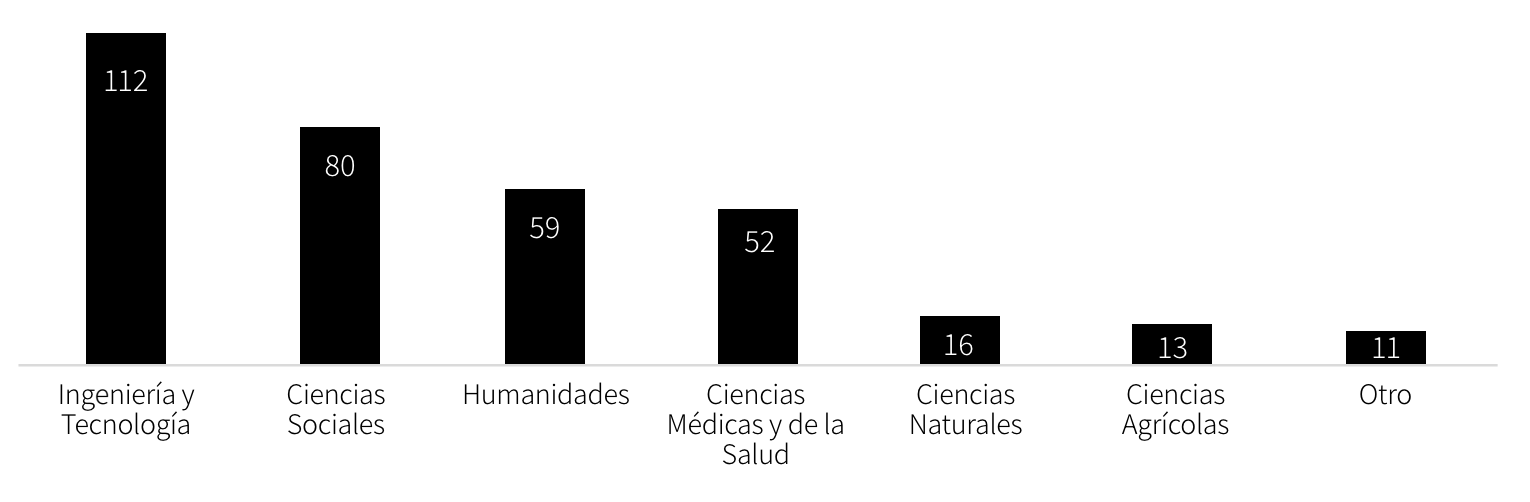
\includegraphics[width=0.7\textwidth,height=\textheight]{img/ingenieria_tecnologia.png}
\caption{Campos de estudio en los que se anticipa mayor crecimiento en
los programas en línea}
\end{figure}

En conclusión, la rápida evolución tecnológica y la transformación del
paisaje educativo presentan una oportunidad singular para innovar en la
entrega de educación en línea. La persistencia de desafíos, como la
estandarización excesiva y la baja tasa de finalización de cursos, no
solo destaca las deficiencias en las plataformas actuales sino que
también subraya el potencial para una plataforma que ofrezca soluciones
personalizadas y adaptativas. Aprovechando las tendencias emergentes y
las necesidades cambiantes del mercado laboral, se revela un campo
fértil para el desarrollo de una oferta educativa que no solo mejore la
experiencia del aprendizaje digital sino que también incremente la
efectividad del mismo. Con el respaldo de datos y proyecciones que
auguran un crecimiento robusto en la demanda de educación técnica en
línea, nuestro proyecto está posicionado estratégicamente para liderar
esta próxima ola de innovación educativa, asegurando que la educación en
línea sea más accesible, relevante y fructífera para todos los
estudiantes.

\newpage

\subsection{3. Entrevista Problema}\label{entrevista-problema}

\subsubsection{3.1 Preguntas}\label{preguntas}

\begin{itemize}
\tightlist
\item
  ¿Cuál es tu edad?

  \begin{enumerate}
  \def\labelenumi{\alph{enumi}.}
  \tightlist
  \item
    Menos de 17 años
  \item
    Entre 17 y 25 años
  \item
    Mayor a 25 años
  \end{enumerate}
\item
  ¿Estás actualmente estudiando?

  \begin{enumerate}
  \def\labelenumi{\alph{enumi}.}
  \tightlist
  \item
    Si
  \item
    No
  \end{enumerate}
\item
  ¿Cuál es tu nivel educativo actual?

  \begin{enumerate}
  \def\labelenumi{\alph{enumi}.}
  \tightlist
  \item
    Primaria
  \item
    Secundaria
  \item
    Universitaria
  \item
    Postgrado
  \item
    otra
  \end{enumerate}
\item
  ¿Qué dificultades has enfrentado con los métodos de enseñanza que
  frecuentas?

  \begin{enumerate}
  \def\labelenumi{\alph{enumi}.}
  \tightlist
  \item
    Falta de personalización
  \item
    Ritmo de aprendizaje inadecuado
  \item
    Dificultad para entender el contenido
  \item
    No he enfrentado dificultades
  \item
    Otra
  \end{enumerate}
\item
  ¿Consideras que tus necesidades individuales de aprendizaje están
  siendo satisfechas?

  \begin{enumerate}
  \def\labelenumi{\alph{enumi}.}
  \tightlist
  \item
    Si
  \item
    No
  \end{enumerate}
\item
  ¿Has utilizado plataformas de educación en línea?

  \begin{enumerate}
  \def\labelenumi{\alph{enumi}.}
  \tightlist
  \item
    Si
  \item
    No
  \end{enumerate}
\item
  ¿Cuánto estarías dispuesto/a a pagar mensualmente en tu educación en
  línea?

  \begin{enumerate}
  \def\labelenumi{\alph{enumi}.}
  \tightlist
  \item
    De 1€ a 15€
  \item
    De 15€ a 30€
  \item
    De 30€ a 50€
  \item
    Más de 50€
  \end{enumerate}
\item
  ¿Te apuntarías a cursos en una plataforma que te deje tener tus
  tiempos y se adapte a tu aprendizaje?

  \begin{enumerate}
  \def\labelenumi{\alph{enumi}.}
  \tightlist
  \item
    Si
  \item
    No
  \end{enumerate}
\end{itemize}

\subsubsection{3.2 Resultados}\label{resultados}

\#\#\#\#\#\#\#\#\#\#\#\#\#\#\#\#\#\#FALTA
COMPLETAR\#\#\#\#\#\#\#\#\#\#\#\#\#\#\#\#\#\#\#\#\#\#\#\#

\newpage

\subsection{4. Mapa de Empatia}\label{mapa-de-empatia}

\subsubsection{4.1. ¿Qué ve?}\label{quuxe9-ve}

Ve desafíos académicos en sus cursos estándar, diferentes estilos de
aprendizaje y la necesidad de obtener buenos resultados académicos.

\subsubsection{4.2. ¿Qué escucha?}\label{quuxe9-escucha}

Escucha la frustración de otros estudiantes por la falta de
personalización en la enseñanza, a profesores sobre el contenido
estándar del curso.

\subsubsection{4.3. ¿Qué piensa y siente?}\label{quuxe9-piensa-y-siente}

Piensa en aprender de manera más efectiva, siente frustración cuando no
puede seguir el ritmo del curso y se preocupa por su desempeño académico
y su futuro profesional.

\subsubsection{4.4. ¿Qué dice y hace?}\label{quuxe9-dice-y-hace}

Expresa su deseo de cursos más adaptados, busca recursos adicionales
para aprender y participa en grupos de estudio o busca ayuda de
compañeros de clase.

\subsubsection{4.5. ¿Cuáles son sus problemas y
necesidades?}\label{cuuxe1les-son-sus-problemas-y-necesidades}

Necesita una educación que se adapte a su estilo de aprendizaje y ritmo,
obtener buenos resultados académicos y herramientas para comprender
mejor los temas difíciles.

\subsubsection{4.6. ¿Qué le motiva?}\label{quuxe9-le-motiva}

La motivación para obtener un título universitario y tener éxito
profesional, aprender nuevas habilidades y superar los desafíos
académicos.

\newpage

\subsection{5. Lienzo de Propuesta de
Valor}\label{lienzo-de-propuesta-de-valor}

\subsubsection{5.1. Tareas del cliente}\label{tareas-del-cliente}

Los clientes buscan obtener información precisa y actualizada, adquirir
habilidades prácticas aplicables y aprender de manera flexible. Esto
implica buscar y seleccionar cursos, inscribirse en ellos, gestionar su
progreso, interactuar con el contenido, participar en evaluaciones,
comunicarse con profesores, colaborar con otros estudiantes y establecer
conexiones. Además, desean mantenerse motivados, desarrollar confianza
en su capacidad y experimentar un sentido de logro al completar cursos y
alcanzar metas personales.

\subsubsection{5.2. Penas del Cliente}\label{penas-del-cliente}

Los clientes pueden enfrentar diversas dificultades al utilizar otra
plataforma, como la frustración por la navegación complicada o la
dificultad para encontrar información específica. También pueden
experimentar preocupación por la sobrecarga de información, temores
relacionados con costos ocultos y la insatisfacción con la calidad del
contenido.

\subsubsection{5.3. Alegrías del Cliente}\label{alegruxedas-del-cliente}

Nuestra plataforma ofrece varias ventajas y alegrías para los clientes.
Estos incluyen el ahorro de tiempo y dinero, y la comodidad. También, la
satisfacción de encontrar contenido relacionado con los intereses y
necesidades del cliente. Además, encontrarán gratificación personal al
alcanzar metas educativas y profesionales.

\subsubsection{5.4. Bienes y Servicios}\label{bienes-y-servicios}

Ofrecemos una amplia gama de servicios y recursos para satisfacer las
necesidades educativas de nuestros clientes. Esto incluye una variedad
de cursos en línea en el área de la tecnología, impartidos por expertos
en la materia, una plataforma intuitiva y fácil de usar con herramientas
interactivas para facilitar el aprendizaje, y un sólido soporte técnico
y académico. Además, nos comprometemos a mantener el contenido
actualizado y a mejorar continuamente nuestra oferta educativa.

\subsubsection{5.5. Creadores de
Alegrías}\label{creadores-de-alegruxedas}

Nuestro equipo se esfuerza por crear una experiencia educativa positiva
y enriquecedora para nuestros clientes. Esto implica ofrecer
flexibilidad en términos de horarios y ubicación, así como la
posibilidad de personalizar el aprendizaje según las preferencias
individuales. También nos comprometemos a proporcionar una amplia
variedad y calidad de contenido educativo, una interfaz intuitiva y
fácil de usar, y una comunidad de apoyo activa para enriquecer la
experiencia de aprendizaje.

\subsubsection{5.6. Quitapenas}\label{quitapenas}

Nos esforzamos por abordar las preocupaciones y dificultades que pueden
surgir al utilizar nuestra plataforma. Esto incluye mejorar la interfaz
y la experiencia del usuario para hacerla más intuitiva y fácil de usar,
así como garantizar la transparencia en los costos y ofrecer un soporte
ampliado. Además, valoramos el feedback de nuestros usuarios y nos
comprometemos a realizar mejoras continuas para satisfacer sus
necesidades y expectativas en términos de calidad y relevancia
educativa.

\newpage

\subsection{6. Modelo de Negocio}\label{modelo-de-negocio}

\subsubsection{6.1. Socios clave}\label{socios-clave}

\begin{itemize}
\tightlist
\item
  Educadores y universidades que proveen cursos y material didáctico.
\item
  Especialistas en tecnología que respaldan la infraestructura de la
  plataforma, incluyendo inteligencia artificial para personalización
  del aprendizaje.
\item
  Organizaciones de Certificación que validan y dan prestigio a los
  certificados ofrecidos por los cursos completados en la plataforma.
\item
  Fuentes financieras que apoyan la sostenibilidad y expansión de la
  plataforma.
\end{itemize}

\subsubsection{6.2. Actividades clave}\label{actividades-clave}

\begin{itemize}
\tightlist
\item
  Actualización de Contenidos: Evaluación y selección de materiales
  educativos que se alineen con las necesidades de los usuarios.
\item
  Marketing y Promoción: Estrategias de marketing digital para atraer a
  nuevos usuarios y retener a los existentes.
\item
  Soporte y Servicio al Cliente: Asistencia continua a usuarios para
  resolver problemas técnicos o dudas académicas.
\end{itemize}

\subsubsection{6.3. Recursos Clave}\label{recursos-clave}

\paragraph{6.3.1. Tangibles}\label{tangibles}

\begin{itemize}
\tightlist
\item
  Físicos: Infraestructura de hardware necesaria para soportar y alojar
  la plataforma de educación en línea, como servidores potentes, equipos
  de cómputo y sistemas de almacenamiento de datos.
\item
  Económicos-financieros: Capital necesario para mantener la plataforma,
  promocionar el servicio educativo y pagar al equipo humano.
\end{itemize}

\paragraph{6.3.2 Intangibles}\label{intangibles}

\begin{itemize}
\tightlist
\item
  Equipo Humano: Un equipo de profesionales que incluye desarrolladores
  web, creadores de contenido, especialistas en marketing, personal de
  soporte y personal educativo.
\item
  Asistencia personal: Ofrecer asistencia individualizada para resolver
  dudas o problemas técnicos.
\item
  Comunidad de Aprendizaje: Crear foros y redes sociales donde los
  estudiantes puedan interactuar entre sí.
\item
  Creación colectiva: Obtener y actuar en base a las opiniones y
  sugerencias de los usuarios para mejorar continuamente la plataforma y
  crear valor.
\end{itemize}

\subsubsection{6.4. Canales}\label{canales}

\paragraph{6.4.1. Tipo de canal}\label{tipo-de-canal}

\begin{itemize}
\tightlist
\item
  Sitio Web Oficial: El principal punto de acceso a los cursos y
  recursos de la plataforma.
\end{itemize}

\paragraph{6.4.2. Fase de canal}\label{fase-de-canal}

\begin{enumerate}
\def\labelenumi{\arabic{enumi}.}
\tightlist
\item
  Información: promoción en redes sociales, eventos y conferencias
  online.
\item
  Evaluación: Descuentos en inscripción a cursos.
\item
  Compra: A través de nuestra página web.
\item
  Entrega: A través de la personalización de cursos en la página web.
\item
  Postventa: Soporte y foros de consulta con profesores.
\end{enumerate}

\subsubsection{6.5. Segmento de clientes}\label{segmento-de-clientes}

Nuestro objetivo es crear valor para cualquier individuo que busque
mejorar sus habilidades, conocimientos y perspectivas a través de una
experiencia educativa en línea personalizada y de alta calidad. En
específico, estudiante, profesionales en busca de capacitación y
personas interesadas en aprendizaje personalizado.

\subsubsection{6.6. Estructura de costos}\label{estructura-de-costos}

\paragraph{6.6.1. Costos por Recurso y
Actividad}\label{costos-por-recurso-y-actividad}

\begin{itemize}
\tightlist
\item
  Costos de desarrollo de la plataforma web.
\item
  Costos de contenido educativo, como el pago a instructores, material
  de curso, derechos de autor y licencias de software.
\end{itemize}

\paragraph{6.6.2. Costos Fijos}\label{costos-fijos}

\begin{itemize}
\tightlist
\item
  Los salarios del personal.
\end{itemize}

\paragraph{6.6.3. Costos Variables}\label{costos-variables}

\begin{itemize}
\tightlist
\item
  Los costos de adquisición de contenido educativo, gastos de marketing
  y publicidad, y comisiones de transacción.
\end{itemize}

\paragraph{6.6.4. Economías de escala}\label{economuxedas-de-escala}

A medida que aumenta el volumen de usuarios y cursos, es posible lograr
economías de escala en áreas como desarrollo de plataforma, adquisición
de contenido y marketing, lo que reduce los costos unitarios.

\subsubsection{6.7. Fuentes de ingreso}\label{fuentes-de-ingreso}

Nuestras principales fuentes de ingresos son las suscripciones de los
clientes para acceder a la plataforma y al contenido educativo, la venta
de cursos individuales, los ingresos por publicidad.

\newpage

\subsection{7. Organización: Organigrama y equipo
promotor}\label{organizaciuxf3n-organigrama-y-equipo-promotor}

\subsubsection{7.1. Organigrama}\label{organigrama}

\begin{figure}
\centering
\includegraphics[width=1\textwidth,height=\textheight]{img/Organigrama.png}
\caption{Organigrama}
\end{figure}

\subsubsection{7.2. Equipo Promotor}\label{equipo-promotor}

\textbf{Azul Noguera} \emph{Estratega Principal (CEO)}

\begin{itemize}
\tightlist
\item
  Experiencia: Más de 10 años en el sector de la educación y la
  tecnología, incluyendo roles de dirección en empresas de e-learning.
\item
  Habilidades Clave: Liderazgo estratégico, visión empresarial, gestión
  de equipos multidisciplinarios, desarrollo de negocios.
\item
  Funciones Asignadas: Toma de decisiones estratégicas, representación
  ante terceros, planificación general del negocio.
\end{itemize}

\textbf{Patricio Guledjian} \emph{Director de Tecnología (CTO)}

\begin{itemize}
\tightlist
\item
  Experiencia: Ingeniero informático con 8 años de experiencia en
  desarrollo web y aplicaciones tecnológicas para la educación.
\item
  Habilidades Clave: Desarrollo de software, gestión de infraestructura
  tecnológica, implementación de inteligencia artificial.
\item
  Funciones Asignadas: Supervisión del desarrollo de la plataforma,
  implementación de tecnologías avanzadas, garantía de calidad y
  seguridad.
\end{itemize}

\textbf{Rocio Gonzalez Cingolani} \emph{Directora de Contenido Educativo
(CCO)}

\begin{itemize}
\tightlist
\item
  Experiencia: Pedagoga con 12 años de experiencia en diseño curricular
  y desarrollo de material educativo.
\item
  Habilidades Clave: Creación de contenido didáctico, adaptación
  curricular, evaluación de aprendizaje.
\item
  Funciones Asignadas: Supervisión de la calidad del contenido,
  selección de cursos y materiales, asegurando el cumplimiento de
  estándares pedagógicos.
\end{itemize}

\newpage

\textbf{Rafael Cabre} \emph{Director de Marketing y Ventas (CMO)}

\begin{itemize}
\tightlist
\item
  Experiencia: Profesional en marketing con 7 años de experiencia en
  estrategias digitales y promoción de servicios educativos.
\item
  Habilidades Clave: Marketing digital, gestión de campañas
  publicitarias, análisis de mercado, desarrollo de marca.
\item
  Funciones Asignadas: Planificación y ejecución de estrategias de
  marketing, captación de usuarios, análisis de datos y rendimiento.
\end{itemize}

\textbf{Ian Costantini} \emph{Director Financiero (CFO)}

\begin{itemize}
\tightlist
\item
  Experiencia: Contador público con más de 15 años de experiencia en
  finanzas corporativas y gestión financiera.
\item
  Habilidades Clave: Análisis financiero, planificación presupuestaria,
  gestión de inversiones, obtención de financiamiento.
\item
  Funciones Asignadas: Elaboración de presupuestos, gestión de flujo de
  caja, análisis de rentabilidad, negociación con inversores y entidades
  financieras.
\end{itemize}

\textbf{Lucila Chaves} \emph{Jefa de Recursos Humanos (HR)}

\begin{itemize}
\tightlist
\item
  Experiencia: Especialista en recursos humanos con más de 13 años de
  experiencia en reclutamiento, capacitación y desarrollo del talento en
  empresas tecnológicas y educativas.
\item
  Habilidades Clave: Gestión de recursos humanos, desarrollo
  organizacional, legislación laboral, comunicación interna.
\item
  Funciones Asignadas: Dirección de las políticas de recursos humanos,
  reclutamiento y selección de personal, desarrollo y capacitación de
  empleados, mantenimiento de un ambiente laboral positivo y productivo.
\end{itemize}

\newpage

\subsection{8. Analisis entorno
competitivo}\label{analisis-entorno-competitivo}

\subsubsection{8.1. Empresas las cuales se dediquen a la misma actividad
o parecida a la
nuestra}\label{empresas-las-cuales-se-dediquen-a-la-misma-actividad-o-parecida-a-la-nuestra}

\begin{enumerate}
\def\labelenumi{\alph{enumi}.}
\item
  Coursera
\item
  Udemy
\item
  Duolingo
\end{enumerate}

\subsubsection{8.2. Descripcion de la competencia y
producto}\label{descripcion-de-la-competencia-y-producto}

\begin{enumerate}
\def\labelenumi{\alph{enumi}.}
\item
  Coursera, fundada en octubre de 2011 por académicos de la Universidad
  de Stanford, es una destacada plataforma de educación en línea
  diseñada para ofrecer cursos masivos abiertos en línea (MOOC, por sus
  siglas en inglés). Actualmente, proporciona 3,943 cursos de pago que
  abarcan una amplia gama de disciplinas---desde idiomas y matemáticas
  hasta tecnología, salud, desarrollo personal, ciencias, artes y
  humanidades---, todos impartidos por universidades de prestigio
  mundial y acompañados de certificaciones reconocidas como el
  Mastertrack Certificate. La inscripción tiene un costo mensual de 54
  dólares estadounidenses, y la plataforma no ofrece reembolso por la
  matrícula. Sin embargo, una de las principales críticas hacia Coursera
  radica en su limitada personalización: la plataforma tiende a ofrecer
  contenido pregrabado que incluye ejercicios de opción múltiple sin
  revisión posterior, lo que puede no satisfacer a usuarios que buscan
  una experiencia de aprendizaje más interactiva y adaptada a sus
  necesidades específicas. Este aspecto representa una oportunidad
  significativa para competidores que puedan integrar sistemas de
  aprendizaje más dinámicos y personalizados.
\item
  Udemy es una prominente plataforma de e-learning establecida en 2010
  en San Francisco, California, EE. UU. Dedicada primordialmente a
  profesionales adultos, Udemy se distingue por ofrecer una extensa
  variedad de cursos en áreas como Desarrollo, Negocios, Informática y
  Software, Productividad en la Oficina, Desarrollo Personal, Diseño,
  Marketing, Estilo de Vida, Fotografía, Salud y Fitness, Música, y
  Enseñanzas Académicas.\\
  A diferencia de los tradicionales MOOC desarrollados por
  universidades, Udemy permite a los creadores independientes
  desarrollar, promocionar y monetizar sus cursos, proporcionándoles
  herramientas esenciales para gestionar y obtener ingresos a través de
  las matrículas. Aunque los cursos de Udemy no equivalen a títulos
  universitarios, son ampliamente reconocidos por mejorar habilidades
  profesionales y personales. La plataforma ofrece los cursos a un
  precio mensual de \$10.99 USD y garantiza una política de reembolso de
  30 días.\\
  Sin embargo, al igual que Coursera, Udemy carece de personalización en
  la experiencia del usuario y ofrece contenidos que no requieren una
  interacción profunda o retroalimentación detallada en las actividades,
  lo que puede limitar la profundidad del aprendizaje y la adaptación a
  las necesidades específicas del estudiante.
\item
  Duolingo, fundada en 2011 por el profesor Luis von Ahn y su estudiante
  Severin Hacker en Pittsburgh, Pensilvania, se ha consolidado como una
  plataforma líder en el aprendizaje de idiomas. Conocida por su enfoque
  gamificado y accesible, Duolingo ofrece cursos en más de 30 idiomas,
  desde ampliamente hablados como el inglés, español y francés, hasta
  idiomas menos comunes como el gaélico escocés y el hawaiano, con una
  suscripción mensual de 7.33 dólares sin posibilidad de reembolso.\\
  La plataforma se distingue por la efectividad y la conveniencia de su
  modelo educativo, que integra el aprendizaje en la rutina diaria de
  los usuarios de una manera atractiva y divertida. Con millones de
  usuarios activos a nivel mundial, Duolingo se mantiene como una de las
  aplicaciones más prominentes y estimadas en el sector del e-learning
  de idiomas.\\
  Las lecciones de Duolingo, conocidas por su brevedad, utilizan una
  variedad de ejercicios interactivos que están diseñados para mejorar
  habilidades lingüísticas como la lectura, escritura, comprensión
  auditiva y expresión oral. Cada lección incluye elementos de juego,
  tales como puntos de experiencia, niveles y vidas, que motivan a los
  usuarios a mantener un aprendizaje continuo y comprometido. Aunque
  Duolingo es ideal para quienes buscan dar sus primeros pasos en un
  nuevo idioma mediante cursos básicos presentados de forma lúdica,
  puede no cubrir necesidades avanzadas de aprendizaje lingüístico.
\end{enumerate}

\begin{longtable}[]{@{}
  >{\raggedright\arraybackslash}p{(\columnwidth - 14\tabcolsep) * \real{0.0776}}
  >{\raggedright\arraybackslash}p{(\columnwidth - 14\tabcolsep) * \real{0.0948}}
  >{\raggedright\arraybackslash}p{(\columnwidth - 14\tabcolsep) * \real{0.0862}}
  >{\raggedright\arraybackslash}p{(\columnwidth - 14\tabcolsep) * \real{0.0603}}
  >{\raggedright\arraybackslash}p{(\columnwidth - 14\tabcolsep) * \real{0.0948}}
  >{\raggedright\arraybackslash}p{(\columnwidth - 14\tabcolsep) * \real{0.2414}}
  >{\raggedright\arraybackslash}p{(\columnwidth - 14\tabcolsep) * \real{0.1466}}
  >{\raggedright\arraybackslash}p{(\columnwidth - 14\tabcolsep) * \real{0.1983}}@{}}
\toprule\noalign{}
\begin{minipage}[b]{\linewidth}\raggedright
Empresa
\end{minipage} & \begin{minipage}[b]{\linewidth}\raggedright
fundación
\end{minipage} & \begin{minipage}[b]{\linewidth}\raggedright
mercados
\end{minipage} & \begin{minipage}[b]{\linewidth}\raggedright
cursos
\end{minipage} & \begin{minipage}[b]{\linewidth}\raggedright
reembolso
\end{minipage} & \begin{minipage}[b]{\linewidth}\raggedright
contenido
\end{minipage} & \begin{minipage}[b]{\linewidth}\raggedright
certificaciones
\end{minipage} & \begin{minipage}[b]{\linewidth}\raggedright
Cliente objetivo
\end{minipage} \\
\midrule\noalign{}
\endhead
\bottomrule\noalign{}
\endlastfoot
udemy & 2010 & mundial & 67561 & si & amplia gama de disciplinas & no &
adultos profesionales \\
coursera & 2011 & mundial & 3943 & no & amplia gama de disciplinas & si
& cualquier edad \\
duolingo & 2011 & mundial & 3880 & no & idiomas & no & cualquier edad \\
\end{longtable}

\paragraph{8.2.1 Precio}\label{precio}

por dolares EEUU

\begin{longtable}[]{@{}ll@{}}
\toprule\noalign{}
Empresa & Precio mensual \\
\midrule\noalign{}
\endhead
\bottomrule\noalign{}
\endlastfoot
Coursera & \$ 54 \\
Udemy & \$ 15 \\
Duolingo & \$ 7.33 \\
\end{longtable}

\paragraph{8.2.2 Ingresos y beneficios.}\label{ingresos-y-beneficios.}

\subparagraph{Ingresos Operativos (facturación): por mil dolares
EEUU}\label{ingresos-operativos-facturaciuxf3n-por-mil-dolares-eeuu}

\begin{longtable}[]{@{}llll@{}}
\toprule\noalign{}
Year & Coursera & Udemy & Duolingo \\
\midrule\noalign{}
\endhead
\bottomrule\noalign{}
\endlastfoot
2023 & 635,764 & 728,937 & 531,109 \\
2022 & 523,756 & 629,097 & 369,495 \\
2021 & 415,287 & 515,657 & 250,772 \\
2020 & 293,511 & 429,899 & 161,696 \\
2019 & 184,411 & 276,327 & 70,760 \\
\end{longtable}

\subparagraph{Beneficios: por mil dolares
EEUU}\label{beneficios-por-mil-dolares-eeuu}

\begin{longtable}[]{@{}llll@{}}
\toprule\noalign{}
Year & Coursera & Udemy & Duolingo \\
\midrule\noalign{}
\endhead
\bottomrule\noalign{}
\endlastfoot
2023 & -111,183 & -107,294 & 16,067 \\
2022 & -170,637 & -153,875 & -59,574 \\
2021 & -143,089 & -80,026 & -60,135 \\
2020 & -65,300 & -77,620 & -15,776 \\
2019 & -46,001 & -69,703 & -13,554 \\
\end{longtable}

\paragraph{8.2.3 Número de empleados.}\label{nuxfamero-de-empleados.}

\begin{longtable}[]{@{}llll@{}}
\toprule\noalign{}
Year & Cousera & Udemy & Duolingo \\
\midrule\noalign{}
\endhead
\bottomrule\noalign{}
\endlastfoot
2023 & 1,295 & 1,443 & 720 \\
2022 & 1,401 & 1,678 & 600 \\
2021 & 1,138 & 1,238 & 500 \\
2020 & 779 & 1,013 & 400 \\
2019 & n.a. & n.a & n.a \\
\end{longtable}

\newpage

\subsection{9. Definición del mercado}\label{definiciuxf3n-del-mercado}

\subsubsection{9.1. Cliente objetivo}\label{cliente-objetivo}

Nuestro servicio está diseñado para ofrecer formación complementaria a
estudiantes universitarios y profesionales que buscan especializarse en
el área tecnológica. Para definir con mayor precisión nuestro mercado
objetivo, nos centraremos en estudiantes universitarios de España que
estén interesados en cursos personalizados y adaptados a sus necesidades
de aprendizaje. Esta estrategia nos permitirá identificar y cuantificar
de manera efectiva a nuestro público objetivo, asegurando que nuestros
cursos respondan específicamente a las demandas y expectativas de este
segmento de mercado. Además, estaremos posicionados para satisfacer las
necesidades educativas actuales y futuras de los estudiantes
universitarios, ayudándoles a complementar sus estudios con habilidades
técnicas relevantes y actualizadas.

\subsubsection{9.2. Métricas}\label{muxe9tricas}

En base al estudio de mercado realizado con la encuesta definida
anteriormente, pudimos extraer varios resultados que nos ayudan a
definir diferentes cuestiones.

\textbf{Métrica de Referencia}

Para obtener esta métrica, utilizamos los resultados de nuestra encuesta
donde preguntamos a los usuarios si estarían dispuestas a recomendar
nuestro producto. Según nuestros hallazgos, el 20\% de los encuestados
estarían dispuestos a recomendar un servicio similar al nuestro.

\#\#\#AGREGAR GRAFICO\#\#\#

\textbf{Métrica de Recurrencia}

La métrica de recurrencia es una medida clave que utilizamos para
evaluar la fidelidad y la retención de nuestros clientes en un modelo de
suscripción mensual. Esta métrica se calcula considerando que cada
cliente que adquiere nuestra suscripción mensual la renueva durante un
periodo mínimo de un año. Por lo tanto, asumimos que cada cliente
renovará su suscripción un total de 12 veces en ese periodo.

La tasa de recurrencia de 12 por usuario sugiere que cada cliente
individual, en promedio, generará ingresos equivalentes a 12 meses de
suscripción durante el primer año de su relación con nuestro servicio.
Esta métrica es fundamental para la planificación financiera y para
comprender el valor del ciclo de vida del cliente en nuestro modelo de
negocio de suscripción mensual.

\subsubsection{9.3. Estudio de mercado}\label{estudio-de-mercado}

\textbf{Precio}

Nuestro análisis exhaustivo del mercado ha revelado que nuestro servicio
se distingue de la competencia por ofrecer una combinación única de
cursos personalizados y un sólido soporte que incluye una
retroalimentación constante.

Lo que nos diferencia significativamente de plataformas como Coursera,
Udemy y Duolingo es la atención personalizada que brindamos a nuestros
usuarios. Nuestros cursos están diseñados para complementar los estudios
universitarios, adaptándose a las necesidades específicas de cada
estudiante. Esto se traduce en un mayor valor percibido por parte de
nuestros clientes, quienes valoran la relevancia y utilidad de nuestros
contenidos en su trayectoria académica.

Además, nuestro servicio ofrece un sólido respaldo a través de una
interacción constante. Proporcionamos ayuda y feedback continuo a
nuestros usuarios, asegurando que puedan maximizar su experiencia de
aprendizaje y obtener resultados concretos en su formación.

Por esta razón, hemos decidido estipular un precio de \$60 dólares
estadounidenses mensuales para la suscripción a nuestro servicio. Esta
tarifa refleja el valor agregado que ofrecemos y está respaldada por la
alta disposición a pagar demostrada por un 80\% de los encuestados en
nuestro estudio de mercado.

\textbf{TAM (Mercado Total)}

Nuestro mercado total (TAM) se define por la cantidad de estudiantes
universitarios en España que podrían beneficiarse de nuestra oferta de
formación complementaria y especializaciones.

Según datos del Ministerio de Universidades de España para el curso
académico 2022-2023, podemos observar la siguiente distribución de
estudiantes: \footnote{FUENTE:
  \href{https://www.universidades.gob.es/wp-content/uploads/2023/06/Principales-resultados_EEU_2022-23.pdf}{Ministerio
  de Universidades de España}}

\begin{longtable}[]{@{}ll@{}}
\toprule\noalign{}
Nivel de estudio & Cantidad de estudiantes \\
\midrule\noalign{}
\endhead
\bottomrule\noalign{}
\endlastfoot
Grado y ciclo & 1.353.347 \\
Master & 276.518 \\
Doctorado & 92.382 \\
Total & \textbf{1.722.247} \\
\end{longtable}

Estos números representan la base potencial de clientes a los que
podemos dirigirnos con nuestro servicio educativo. Esta información
respalda nuestra estrategia de mercado y nos proporciona una visión
clara del alcance y la oportunidad dentro del sector universitario
español.

\textbf{SAM (Mercado Objetivo)}

Para determinar nuestro SAM (Servicio Total Disponible), utilizamos los
resultados de encuestas exhaustivas que nos proporcionaron una
estimación realista del porcentaje de alumnos universitarios dispuestos
a consumir nuestro servicio. A partir de estos datos, identificamos que
aproximadamente el 80\% de los encuestados mostraron disposición a pagar
el precio que hemos establecido.

Basándonos en esta información, calculamos nuestro mercado objetivo
inicial tomando el total de estudiantes universitarios en España, que es
de 1.722.247, y aplicando el porcentaje de disposición a pagar (80\%).
Por lo tanto, nuestro SAM se estima en 1.722.247 x 80\% = 1.377.797
potenciales usuarios. Este cálculo nos proporciona una base sólida para
comprender la demanda inicial de nuestro servicio entre los estudiantes
universitarios en España que valoran la formación complementaria y
especializada que ofrecemos. Estamos enfocados en capturar una parte
significativa de este mercado objetivo inicial, aprovechando la
disposición de la mayoría de los estudiantes encuestados a invertir en
nuestra propuesta de valor.

\#\#\#AGREGAR GRAFICO\#\#\#

\textbf{SOM (Mercado Obtenible)}

\#\#\#\#\#\#\#\#\#\#\#\#\#\#\#\#\#\#\#\#\#\#\#\#\#\#\#\#\#\#\#\#\#\#\#\#\#\#\#\#\#\#\textbf{FALTA}\#\#\#\#\#\#\#\#\#\#\#\#\#\#\#\#\#\#\#\#\#\#\#\#\#\#\#\#\#\#\#\#\#\#\#\#\#\#\#\#\#\#

La capacidad de tus servidores y el ancho de banda disponible para
determinar cuántos estudiantes simultáneos puedes atender de manera
efectiva.

\newpage

\subsection{10. Marketing}\label{marketing}

\subsubsection{10.1. Medios que usaremos para vender el
producto}\label{medios-que-usaremos-para-vender-el-producto}

\textbf{Facebook}

\begin{itemize}
\tightlist
\item
  Interacción Orgánica: Nos comprometemos a mantener una presencia en
  línea sólida y dinámica a través de nuestra página oficial, la cual
  será gestionada por un Community Manager altamente capacitado. Este
  profesional se encargará de garantizar un flujo constante de
  publicaciones diarias que se centrarán en dos áreas cruciales: la
  comunicación clara y convincente de nuestra propuesta de valor única,
  resaltando los aspectos diferenciadores de nuestro producto en el
  mercado; y la publicación de contenido relevante y actualizado
  relacionado con la educación y el estudio.
\item
  Publicidad Pautada: Implementaremos una estrategia publicitaria
  pautada en Facebook para potenciar el alcance y la visibilidad de
  nuestra plataforma. A través de campañas cuidadosamente diseñadas,
  buscaremos generar un crecimiento acelerado y dirigir un flujo
  constante de tráfico hacia nuestro sitio web.
\end{itemize}

\textbf{Instagram}

\begin{itemize}
\tightlist
\item
  Publicaciones Diarias: Trabajaremos en estrecha colaboración con
  nuestro Community Manager para desarrollar y mantener una programación
  de publicaciones diarias. Estas publicaciones se centrarán en
  transmitir nuestra propuesta de valor de manera efectiva, priorizando
  contenido visual de alta calidad, especialmente videos, para captar la
  atención de nuestra audiencia.
\item
  Campañas Dirigidas a Educadores: Implementaremos campañas
  publicitarias específicas dirigidas a educadores, destacando los
  beneficios clave de nuestra plataforma mediante comparaciones con
  métodos de enseñanza tradicionales. Enfocaremos nuestros esfuerzos en
  resaltar cómo nuestra solución puede mejorar la eficiencia, la
  interacción y los resultados en el proceso de enseñanza-aprendizaje.
\item
  Campañas Dirigidas a Alumnos: Asimismo, dirigiremos campañas
  publicitarias específicas hacia los potenciales alumnos. En estas
  campañas, pondremos énfasis en los beneficios tangibles que ofrecemos,
  como la capacidad de grabar clases, la seguridad de la plataforma y la
  disponibilidad de profesores altamente cualificados. Estos aspectos se
  presentarán de manera convincente para mostrar cómo nuestra plataforma
  puede mejorar significativamente la experiencia de aprendizaje para
  los estudiantes.
\end{itemize}

\textbf{Google Ads}

\begin{itemize}
\tightlist
\item
  Campaña de Palabras Clave: Desarrollaremos una campaña publicitaria
  enfocada en capturar la búsqueda de palabras clave relevantes para
  nuestro sector, tales como ``clases particulares'' y ``educadores
  particulares'', entre otros términos clave. Esta estrategia nos
  permitirá posicionarnos de manera destacada en los resultados de
  búsqueda y llegar a una audiencia altamente motivada en su búsqueda de
  soluciones educativas.
\item
  Constante Evaluación y Optimización: Nos comprometemos a realizar una
  evaluación continua de nuestra campaña publicitaria en Google Ads para
  garantizar una generación efectiva de tráfico hacia nuestro sitio web.
  Esto implicará un monitoreo constante de los datos de rendimiento y la
  realización de ajustes estratégicos según sea necesario para maximizar
  el impacto y la eficacia de nuestra inversión publicitaria.
\end{itemize}

\subsubsection{10.2. Costo de la promocion}\label{costo-de-la-promocion}

En nuestro análisis de costos, emplearemos el modelo del Costo por Mil
Impresiones (CPM), una métrica fundamental en la publicidad en línea,
que cuantifica el costo que los anunciantes incurren por cada mil
impresiones de sus anuncios. Esta métrica nos permite evaluar el alcance
y la efectividad de nuestras campañas publicitarias, ofreciendo una
visión integral de nuestra inversión en marketing digital.

\textbf{Facebook Ads}

Según los datos proporcionados por Neo Attack \footnote{FUENTE:
  \href{https://neoattack.com/blog/cuanto-cuesta-facebook-ads/\#:~:text=tipo\%20de\%20empresas.-,Cu\%C3\%A1nto\%20cuesta\%20Facebook\%20Ads\%20en\%20Espa\%C3\%B1a,entre\%200.5\%20y\%203\%E2\%82\%AC.}{¿Cuánto
  cuesta Facebook Ads?}}, el CPM de una campaña en Facebook en España
generalmente oscila entre 2 y 5€.

\textbf{Instagram Ads}

De acuerdo con la información de Dinamiza Digital \footnote{FUENTE:
  \href{https://dinamizadigital.com/cuanto-cuesta-la-publicidad-en-instagram/}{Cuánto
  cuesta la publicidad en Instagram en España?}}, el CPM promedio en
España para Instagram Ads varía entre 1,97€ y 5,39€.

\textbf{Google Ads}

Aunque no se proporciona un dato específico para el CPM de Google Ads en
España en los enlaces proporcionados, se puede inferir que el CPM en
España para Google Ads podría estar en un rango similar al global,
alrededor de \$2.40.

Es importante tener en cuenta que estas cifras son estimaciones
aproximadas y que el costo real puede variar según diversos factores,
como la audiencia objetivo, el formato del anuncio y la competencia en
el mercado. Para obtener una estimación más precisa, es recomendable
considerar la colaboración con una agencia de marketing digital o el uso
de herramientas especializadas.

\subsubsection{10.3. Estimacion de personas atraidas por la
promocion}\label{estimacion-de-personas-atraidas-por-la-promocion}

Los conversion rates y los click-through rates (CTR) en las plataformas
publicitarias clave como Facebook Ads, Google Ads e Instagram Ads pueden
variar significativamente. Se observa que:

\textbf{Facebook Ads}

Según Wordstream, una cadena de marketing, la tasa de conversión
promedio en Facebook Ads para el sector educativo se sitúa en torno al
13.58\% \footnote{FUENTE:
  \href{https://www.wordstream.com/blog/ws/2017/02/28/facebook-advertising-benchmarks}{Facebook
  Ad Benchmarks for YOUR Industry.}}. Este nivel de conversión refleja
la capacidad de Facebook para atraer y comprometer a audiencias
educativas, destacando su eficacia como un canal publicitario relevante
para las instituciones educativas. Además, el CTR para Facebook Ads es
del 0.73\% \footnote{FUENTE:
  \href{https://www.wordstream.com/blog/ws/2017/02/28/facebook-advertising-benchmarks}{Facebook
  Ad Benchmarks for YOUR Industry.}}, lo que indica la proporción de
usuarios que hacen clic en un anuncio después de verlo.

\begin{figure}
\centering
\includegraphics[width=0.8\textwidth,height=\textheight]{img/facebook.png}
\caption{La tasa de conversion de todas las industrias de Facebook Ads.}
\end{figure}

\textbf{Google Ads}

En el caso de Google Ads, la tasa de conversión promedio para el sector
educativo se sitúa alrededor del 5.93\% para la búsqueda (Search)
\footnote{FUENTE:
  \href{https://www.wordstream.com/blog/ws/2022/05/18/search-advertising-benchmarks}{2022
  Google Ads \& Microsoft Ads Benchmarks for Every Industry.}}. Esta
plataforma también muestra un rendimiento sólido en términos de
conversion rates para las instituciones educativas que utilizan sus
servicios publicitarios. El CTR para Google Ads es del 6.17\%
\footnote{FUENTE:
  \href{https://www.wordstream.com/blog/ws/2022/05/18/search-advertising-benchmarks}{2022
  Google Ads \& Microsoft Ads Benchmarks for Every Industry.}}, lo que
indica una alta interacción de los usuarios con los anuncios en los
resultados de búsqueda y en sitios web asociados.

\textbf{Instagram Ads}

Aunque los datos específicos para el sector educativo no están
disponibles, es importante tener en cuenta que el conversion rate
promedio para Instagram Ads se sitúa en aproximadamente el 1.08\%
\footnote{FUENTE:
  \href{https://visme.co/blog/es/instagram-ads/}{Instagram Ads: ¿Cómo
  crearlos en 2023 para convertir?}}. Respecto al CTR para Instagram
Ads, este se encuentra en el 0.52\% \footnote{FUENTE:
  \href{https://lorenzo-gonzalez.com/instagram-analytics-las-9-metricas-mas-importantes-para-medir-tu-exito/\#:~:text=Tasas\%20de\%20clics\%20de\%20anuncios\%20(CTR),-El\%20objetivo\%20principal&text=Las\%20tasas\%20de\%20clics\%20promedio,\%2C52\%25\%2Cseg\%C3\%BAn\%20Adstage.}{Instagram
  Analytics}}.

\textbf{Estimación de Conversion Rate Final}

Al promediar las tasas de conversión de Facebook Ads (13.58\%), Google
Ads (5.93\%) e Instagram Ads (1.08\%) para el sector educativo,
obtenemos una estimación de la tasa de conversión final de
aproximadamente el 6.86\%. Esta cifra combinada ofrece una visión
general de la posible efectividad de nuestras campañas publicitarias en
estas plataformas para promocionar servicios educativos.

Es crucial tener en cuenta que las tasas de conversión y los CTR pueden
variar según diversos factores, como la estrategia de marketing, la
calidad del contenido y la relevancia de las campañas publicitarias en
cada plataforma. Por lo tanto, es esencial realizar un seguimiento
continuo y ajustar nuestras estrategias según los resultados obtenidos
para maximizar el rendimiento de nuestras inversiones en publicidad
digital en el sector educativo.

\newpage

\subsection{11. Produccion y
operaciones}\label{produccion-y-operaciones}

\subsubsection{11.1 Servicio Minimo Viable y
localizacion}\label{servicio-minimo-viable-y-localizacion}

\textbf{Desarrollo de Cursos Originales} Crearemos cursos de tecnología
completamente originales, diseñados internamente por nuestro equipo
experto. Estos cursos se adaptarán a diferentes estilos de aprendizaje e
intereses de los usuarios, permitiendo una mayor personalización y
relevancia.

\textbf{Aprendizaje Adaptativo Básico} Implementaremos funcionalidades
de aprendizaje adaptativo que ajusten el nivel de dificultad y el ritmo
del curso según el progreso del estudiante. Este proceso inicialmente
será supervisado por instructores y evolucionará hacia un enfoque más
automatizado con algoritmos simples.

\textbf{Encuestas de Retroalimentación} Realizaremos encuestas
periódicas para recopilar información detallada sobre la experiencia de
aprendizaje de los estudiantes. Esto nos permitirá identificar áreas de
mejora y adaptar de manera personalizada el contenido y la estructura de
nuestros cursos.

\textbf{Comunidad} Facilitaremos un espacio interactivo donde los
estudiantes puedan conectar entre sí y con los instructores. Este
entorno permitirá discusiones, intercambio de recursos y brindará una
plataforma para recibir retroalimentación directa sobre la experiencia
de aprendizaje.

Con este enfoque, lanzaremos un producto inicial sólido que destaque por
la calidad y la personalización de nuestros cursos originales. A medida
que obtengamos retroalimentación y validemos nuestro enfoque, podremos
expandirnos a otras áreas de aprendizaje y mejorar la funcionalidad de
la plataforma.

\subsubsection{11.2. Instalaciones, Medios y
Equipos}\label{instalaciones-medios-y-equipos}

\textbf{Medios Técnicos:}

\begin{itemize}
\item
  Servidores de Alta Capacidad: Para garantizar la escalabilidad y
  robustez de nuestra plataforma de educación en línea, se adquirirán
  tres servidores HP ProLiant ML350 Gen10. Estos servidores son
  conocidos por su alta capacidad de procesamiento y expansión, lo que
  los hace ideales para manejar grandes volúmenes de datos y
  transacciones en tiempo real. Estarán ubicados en las instalaciones de
  uno de nuestros socios tecnológicos, lo que minimiza la necesidad de
  espacio físico adicional y reduce costos operativos. El costo de cada
  servidor es aproximadamente de \$5,000, sumando un total de \$15,000
  para la adquisición inicial.
\item
  Equipos Informáticos: Utilizaremos los equipos personales de nuestro
  equipo técnico, que ya cuentan con las especificaciones necesarias
  para el desarrollo y mantenimiento de aplicaciones de alta demanda.
  Esta estrategia reduce la inversión inicial en hardware y permite una
  mayor flexibilidad operativa.
\end{itemize}

\textbf{Infraestructura:}

\begin{itemize}
\tightlist
\item
  Red de Internet de Alta Velocidad: Esencial para el acceso sin
  interrupciones y el funcionamiento eficaz de la plataforma, contamos
  con un servicio de internet de fibra óptica que ofrece velocidades
  óptimas para el desarrollo y la entrega de contenido en línea. Esto es
  crucial para el trabajo remoto del equipo y la experiencia del usuario
  final.
\end{itemize}

\textbf{Tecnología:}

\begin{itemize}
\tightlist
\item
  Inteligencia Artificial (IA): Bajo la dirección de nuestro
  especialista en tecnología, desarrollaremos algoritmos avanzados de IA
  que permitirán personalizar la experiencia de aprendizaje de los
  estudiantes. Estos algoritmos estarán diseñados para analizar el
  progreso del usuario y adaptar el contenido educativo de manera
  proactiva, mejorando así la retención del conocimiento y la
  satisfacción del estudiante. Esta inversión no solo refuerza nuestro
  compromiso con la educación personalizada sino que también coloca a
  nuestra plataforma a la vanguardia de la innovación tecnológica en
  educación.
\end{itemize}

\textbf{Inversión:}

\begin{itemize}
\tightlist
\item
  Costos de Implementación: Además de la compra de los servidores, se
  invertirán aproximadamente \$1,000 en la instalación y configuración
  inicial, asegurando que la infraestructura tecnológica esté
  óptimamente preparada para soportar nuestras operaciones desde el
  inicio.
\end{itemize}

\begin{longtable}[]{@{}
  >{\raggedright\arraybackslash}p{(\columnwidth - 4\tabcolsep) * \real{0.4105}}
  >{\raggedright\arraybackslash}p{(\columnwidth - 4\tabcolsep) * \real{0.4211}}
  >{\raggedright\arraybackslash}p{(\columnwidth - 4\tabcolsep) * \real{0.1684}}@{}}
\toprule\noalign{}
\begin{minipage}[b]{\linewidth}\raggedright
Categoría
\end{minipage} & \begin{minipage}[b]{\linewidth}\raggedright
Detalle
\end{minipage} & \begin{minipage}[b]{\linewidth}\raggedright
Costo (USD)
\end{minipage} \\
\midrule\noalign{}
\endhead
\bottomrule\noalign{}
\endlastfoot
Servidores de Alta Capacidad & 3 x HP ProLiant ML350 Gen10 & \$15,000 \\
Instalación y Configuración & Configuración inicial de servidores &
\$1,000 \\
\textbf{Total Estimado} & & \textbf{16,000} \\
\end{longtable}

Esta planificación estratégica de la inversión en infraestructura
tecnológica crea una base sólida para el lanzamiento y la expansión de
nuestra plataforma educativa en línea. Al invertir en servidores de alta
capacidad y desarrollar internamente nuestras soluciones de IA, estamos
asegurando que nuestra plataforma no solo cumpla con los requisitos
actuales de los usuarios sino que también esté preparada para adaptarse
a las necesidades futuras, proporcionando así una experiencia educativa
en línea superior y altamente confiable.

\subsubsection{11.3. Sistema de
operaciones}\label{sistema-de-operaciones}

\textbf{Planificación Estratégica} - Definir objetivos claros para el
MVP, incluyendo las funcionalidades esenciales que se deben implementar.
- Establecer un cronograma detallado con hitos específicos para el
desarrollo y lanzamiento. - Desarrollo e Implementación de la Plataforma
Web

\textbf{Desarrollo de Contenido de Cursos} - Diseño y desarrollo de
módulos educativos interactivos por parte de nuestros expertos en
creación de contenido. - Integración de multimedia y recursos
interactivos para mejorar la experiencia de aprendizaje. - Revisión y
validación del contenido por expertos en la materia para garantizar su
calidad y relevancia.

\textbf{Aprobación y Publicación} - Realizar pruebas exhaustivas de la
plataforma y los contenidos para asegurar su funcionalidad y precisión.
- Obtener las aprobaciones necesarias de las partes interesadas para
asegurar que el producto cumple con las expectativas y requisitos
reglamentarios. - Publicar el contenido en la plataforma, asegurando que
esté accesible y optimizado para diferentes dispositivos.

\textbf{Lanzamiento de los Cursos} - Planificar una estrategia de
lanzamiento que incluya eventos promocionales y colaboraciones con
influencers o expertos del sector. - Monitorear la respuesta de los
usuarios y ajustar rápidamente cualquier aspecto del servicio según sea
necesario.

\textbf{Marketing y Publicidad} - Desarrollar y ejecutar una campaña de
marketing digital para crear conciencia y atraer a los usuarios
objetivo. - Utilizar estrategias de marketing de contenidos, publicidad
pagada y redes sociales para maximizar el alcance y la captación. -
Establecer métricas de seguimiento para evaluar el impacto de las
actividades de marketing y ajustar las tácticas en función de los
resultados obtenidos.

\newpage

\end{document}
